\documentclass[11pt,a4paper]{article}
\usepackage[utf8]{inputenc}
\usepackage[T1]{fontenc}
\usepackage[english]{babel}
\usepackage{lmodern}
\usepackage{microtype}
\usepackage{geometry}
\usepackage{graphicx}
\usepackage{xcolor}
\usepackage{hyperref}
\usepackage{tikz}
\usetikzlibrary{arrows.meta,positioning}

% Ajustes básicos de estilo
\geometry{margin=2.5cm}
\setlength{\parskip}{0.6em}
\setlength{\parindent}{0pt}
\graphicspath{{./figuras/}}
\hypersetup{
  colorlinks=true,
  linkcolor=blue!60!black,
  urlcolor=blue!60!black,
  citecolor=blue!60!black
}

\title{Implementation of custom HMM for Basque and Catalan}
\author{Josu Bayer, Ane Paniagua, Ander Pe\~na, Be\~nat Alkain}
\date{\today}

\begin{document}
\maketitle
\tableofcontents
\bigskip

\section{Introduction}
Part-of-speech tagging assigns a syntactic role to each token (e.g., DET, NOUN, VERB) so that well-formed transitions such as ADJ\,$\rightarrow$\,NOUN or NOUN\,$\rightarrow$\,VERB emerge while unlikely ones are penalized. In this project we frame tagging as a generative sequence problem with Hidden Markov Models, estimating joint probabilities \(p(x, y) = p(y)\,p(x\mid y)\) over words and tags. Transition probabilities capture contextual constraints between tags, and emission probabilities capture how likely a word is given its tag under the Markov and output-independence assumptions.

Our goal is to implement and evaluate a custom HMM tagger on two Universal Dependencies corpora (Basque and Catalan) to test robustness across a highly agglutinative language and a more fusional one. We compare against the reference HMM in \texttt{nltk} and backoff n-gram baselines (unigram, bigram, trigram), using token-level accuracy on train/dev/test and per-tag breakdowns over the 17 universal categories. This report follows the grading axes: correct HMM implementation, sound experiments on two datasets, and analysis of results.

\section{Methodology}
We use the Universal Dependencies corpora for Basque and Catalan, each provided as CSV with parallel \textit{text} and \textit{tags} fields. Sentences are tokenized at whitespace and paired word-by-word with their UPOS labels (17-tag inventory). Data are split into train/dev/test partitions; train drives parameter estimation, dev is used for model comparison, and test reports final generalization. Table~\ref{tab:csv-ud} shows sample rows from the Basque training split to illustrate the schema and the morpho-syntactic granularity of the tags.

\begin{table}[h]
  \centering
  \caption{UD CSV structure (Basque train split).}
  \label{tab:csv-ud}
  \small
  \begin{tabular}{p{2cm}p{4cm}p{9cm}}
    \hline
    sentence\_id & text & tags \\
    \hline
    train-s1 & Gero , lortutako masa molde batean jarri . & ADV PUNCT VERB NOUN NOUN NUM VERB PUNCT \\
    train-s2 & Bestalde , `` herri palestinarrari laguntza tekniko eta ekonomikoa ematen jarraitzeko ... baieztatu zuen EBk . & CCONJ PUNCT NOUN ADJ NOUN ADJ CCONJ ADJ VERB VERB CCONJ NOUN ADJ CCONJ ADJ NUM NOUN AUX NOUN ADJ VERB NOUN VERB NOUN PUNCT VERB AUX PROPN PUNCT \\
    \hline
  \end{tabular}
\end{table}

The core model is a Hidden Markov Model that factorizes the joint sequence probability as \(p(x, y) = p(y)\,p(x\mid y)\). Transition probabilities \(p(y_i\mid y_{i-1})\) and emission probabilities \(p(x_i\mid y_i)\) are estimated by maximum likelihood counts over the training set, with explicit initial-state probabilities for sentence starts. The MLE parameter estimation and Viterbi decoding are implemented in \texttt{model/hmm.py} (methods \texttt{train} and \texttt{viterbi}), and the evaluation helpers for accuracy and per-tag accuracy live in \texttt{main.py}.

To ground results, we train two implementations: (i) the reference \texttt{nltk} HMM tagger; (ii) our own HMM implementation using the same MLE recipe and Viterbi decoding as above. We also build backoff n-gram baselines (default, unigram, bigram, trigram) to quantify the benefit of sequential context over context-free tagging.

Evaluation is token-level accuracy on train/dev/test for both languages, complemented with per-tag accuracy to identify categories with higher error (e.g., infrequent or ambiguous tags). We also inspect POS frequency distributions to anticipate sparsity effects, and run qualitative Viterbi examples to verify that predicted tag transitions align with plausible syntactic sequences.

\begin{figure}[h]
  \centering
  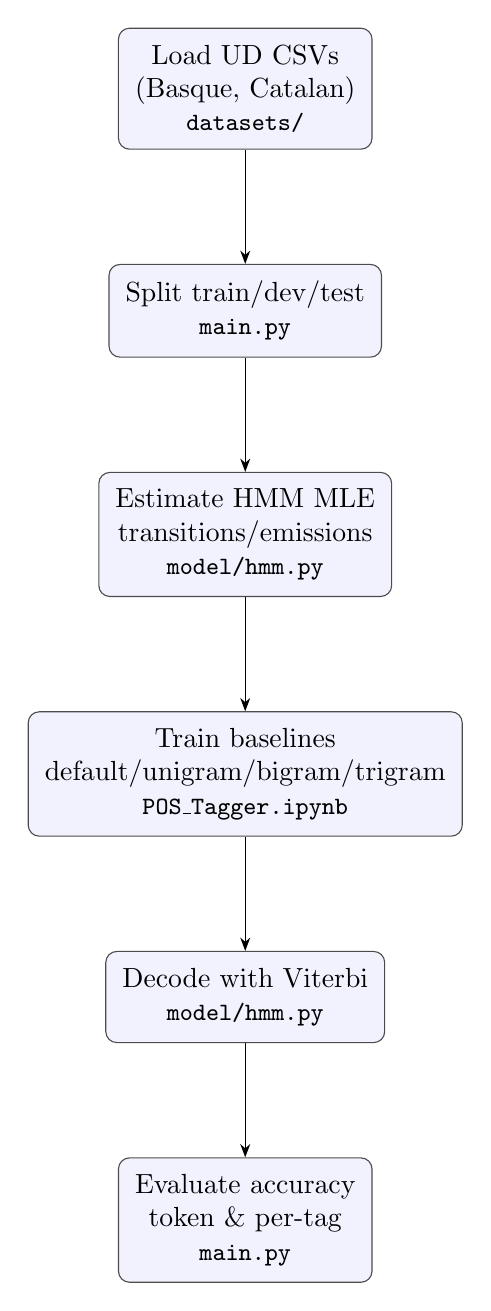
\begin{tikzpicture}[>=Stealth, node distance=1.45cm, every node/.style={rectangle, rounded corners, draw=black!70, fill=blue!5, align=center, inner sep=6pt}]
    \node (load) {Load UD CSVs\\(Basque, Catalan)\\\small \texttt{datasets/}};
    \node (split) [below=of load] {Split train/dev/test\\\small \texttt{main.py}};
    \node (train) [below=of split] {Estimate HMM MLE\\transitions/emissions\\\small \texttt{model/hmm.py}};
    \node (baseline) [below=of train] {Train baselines\\default/unigram/bigram/trigram\\\small \texttt{POS\_Tagger.ipynb}};
    \node (decode) [below=of baseline] {Decode with Viterbi\\\small \texttt{model/hmm.py}};
    \node (eval) [below=of decode] {Evaluate accuracy\\token \& per-tag\\\small \texttt{main.py}};
    \draw[->] (load) -- (split);
    \draw[->] (split) -- (train);
    \draw[->] (train) -- (baseline);
    \draw[->] (baseline) -- (decode);
    \draw[->] (decode) -- (eval);
  \end{tikzpicture}
  \caption{Methodological flow: data ingestion to evaluation with code pointers.}
\end{figure}

\section{Results}
% Key metrics, tables, figures, and error analysis.



\section{Conclusions}
% Main findings and future work.

\end{document}
